\section{Network of \emph{parameterization prediction}}
In this section, we first explain the general framework of our proposed network in Sec~\ref{subsec:overview}, and then we elaborate the details of its structure part by part in the following sections.

\begin{figure}[htbp]
	\centering
	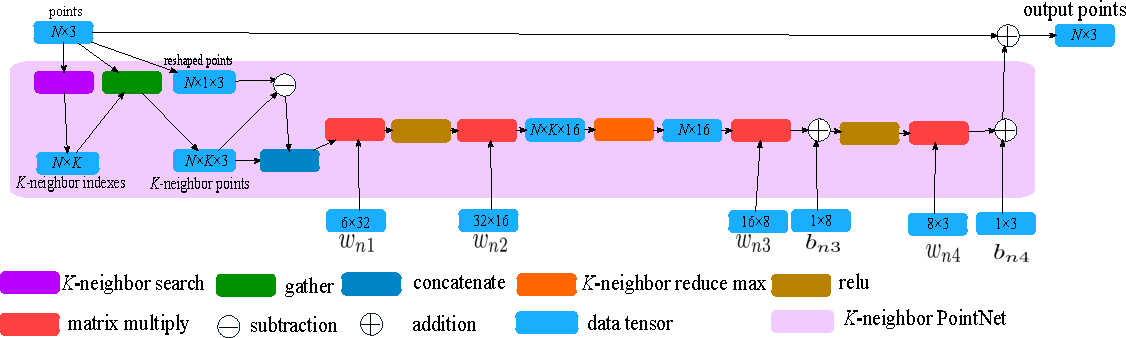
\includegraphics[width=\linewidth]{img/net/k-n_pointnet}
	\caption{The internal structure of \textit{K}-neighbor PointNet}
	\label{fig:knpointnet}
\end{figure}

\subsection{Network overview}
\label{subsec:overview}
Our original idea about network of \emph{parameterization prediction} was to use a semantic network that takes image as input to predict a mapping from the parameter domain to the target surface. In the proposed framework shown in Figure~\ref{fig:overview}, the mapping is actually expressed by the parameterization network. Instead of directly predicting the mapping, the semantic network predicts parameters for the parameterization network, making the entire network end-to-end trainable.

The parameterization network is built by stacking several \textit{K}-neighbor PointNet (explained in Sec~\ref{subsec:k-n_point_net}). Each \textit{K}-neighbor PointNet takes point set as input and predicts a offsets for each point and add them to the input points. In this way, the parameterization network can map/deform a randomly sampled point set to target shape. By using different randomly generated samples from the parameter domain in the training iterations, the parameterization network can learn to handle the \textit{sampling variation} that is introduced by using specific point set as ground truth. 

The semantic network is built on convolution, deconvolution and fully connected layers, it takes image as input to predict the parameters (i.e.$\{P_1,P_2,P_3,P_4,P_5\}$ in Figure~\ref{fig:overview}) for the parameterization network. In this way, the semantic network relates the input image to the parameterization.

\begin{figure*}[htbp]
	\centering
	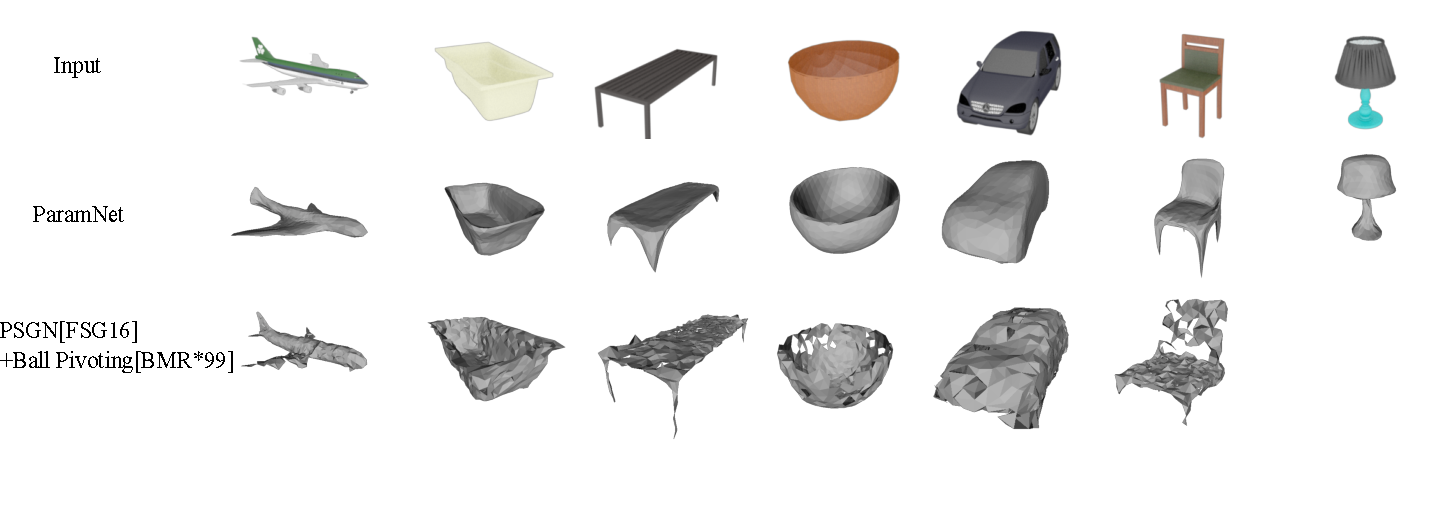
\includegraphics[width=\linewidth]{img/res/res}
	\caption{The comparison of visual results}
	\label{fig:res}
\end{figure*}

\subsection{Parameter domain}
In the proposed framework, we use unit sphere surface as parameter domain. As shown in Figure~\ref{fig:overview}, at the beginning of the parameterization network $N=1024$ points are uniformly sampled from the parameter domain. Triangulation is also applied on these sampled points. The edge connections built by triangulation are later used in the Laplacian smooth layer and the edge length regularization term. These connections are also used to connect output points to mesh.
\subsection{\textit{K}-neighbor PointNet for parameterization network} 
\label{subsec:k-n_point_net}

\begin{figure*}[htbp]
	\centering
	\includegraphics[width=\linewidth]{img/abl/abl}
	\caption{Visual result for ablation study: In some cases, the view angle is adjusted for better exposure of imperfection}
	\label{fig:abl}
\end{figure*}

\begin{table*}
	\caption{Ablation study with respect to different components}
	\label{tab:ablation}
	\centering
	\begin{tabular}{c | c c c c c}
		Models &  Full Model  & -Initialization & -Laplation smooth & -Edge length regularization & -Norm loss \\
		\hline
		Chamfer      & 0.297 & 0.424 & 0.394 & 0.405  & 0.390\\
		EMD			 & 0.834 & 1.524 & 1.369 & 4.195  & 1.415
	\end{tabular}
\end{table*}

An essential building block for our parameterization network is \textit{K}-neighbor PointNet. Figure~\ref{fig:knpointnet} shows the structure of \textit{K}-neighbor PointNet. \textit{K}-neighbor PointNet is inspired by and named after PointNet\cite{PointNet} and its follow-up PointNet++\cite{NIPS2017_7095}. In order to take unordered point set as input, \textit{K}-neighbor PointNet uses either point-wise operations on each point or symmetric functions on multiple points. As shown in Figure~\ref{fig:knpointnet}, the \textit{K}-neighbor search operation finds the $K$ neareast neighbor point for each point inside the $N$ input points and output the indexes tensor. We employed the Bitonic Sort\cite{bitonicsorter} for its implementation on GPU. Then the  \emph{gather} operation forge the tensor of \textit{K}-neighbor points based on these indexes and input points. This operation is tensorflow  Subtracting the original input points from \textit{K}-neighbor points we can get the local relative coordinates of \textit{K}-neighbor points. By concatenating \textit{K}-neighbor point coordinates and their local relative coordinates, we get the $N\times K\times6$ tensor as geometric features. These features go through a series of operations as shown in Figure~\ref{fig:knpointnet} to predict point-wise 3D offsets for each input point. Unlike the original PointNet\cite{PointNet}, who extracts maximum value among all point as feature vector for input point set, our \textit{K}-neighbor PointNet extract maximum value among every \textit{K}-neighborhood as feature vector for each point. This is shown by the \textit{K}-neighbor reduce max operation in Figure~\ref{fig:knpointnet}.

\subsection{Laplacian smooth}
Another essential building block for our parameterization network is the Laplacian smooth layer. Mesh based Laplacian smooth is commonly used in mesh processing. The Laplacian smooth layer applys the mesh based Laplacian smooth operation for each point in the point set as in (\ref{equ:lpl}). The mesh is constructed by triangulation on the sample points from parameter domain (i.e. the unit sphere surface). In (\ref{equ:lpl}), $\mathcal{N}(\mathbf{x})$ represents the one-ring neighborhood of $\mathbf{x}$. As described in (\ref{equ:lpl}), the Laplacian smooth is a local linear operation and therefore differentiable.

\begin{equation}
\mathbf{x^*} = \frac{1}{|\mathcal{N}(\mathbf{x})|}\sum_{\mathbf{y}\in\mathcal{N}(\mathbf{x})}\mathbf{y}
\label{equ:lpl}
\end{equation}

Our ablation study shows that the Laplacian smooth significantly improves the regularity of the generated surface and makes the output mesh visually much more appealing. It also prevent self-intersection of the surface locally
\subsection{Semantic network}
\label{subsec:semnet}
In our semantic network, we use convolution layers to extract semantic features from input image as shown in Figure~\ref{fig:semnet}.  Our semantic network adopt the U-shape structure that is similar to UNet\cite{unet}. To fit with our framework, we use separate decoder branches to predict different parameters parameterization network. These predicted parameters (i.e. $P_n=\{w_{n1},w_{n2},w_{n3},b_{n3},w_{n4},b_{n4},s_{n}\}$ ) are plugged into the parameterization network in the way shown in Figure~\ref{fig:overview}

\subsection{Losses}
The whole loss we use is shown in Eq.(\ref{equ:loss}), it is composed of the four terms as follows:
\begin{equation}
\label{equ:loss}
l = l_c + \alpha l_2 + \beta l_{reg} + l_n
\end{equation}

\noindent{\textbf{Chamfer loss}} The Chamfer distance is directly borrowed from \cite{PSGN}. This loss can drive the output point set to approach the target. As shown in Eq.(\ref{equ:chmf}). In Eq.(\ref{equ:chmf}), $\mathbf{x}$ are output points and $\mathbf{y}$ are the points from the groundtruth

\begin{equation}
\label{equ:chmf}
l_c = \sum_\mathbf{x} \min||\mathbf{x}-\mathbf{y}||_2^2+\sum_\mathbf{y} \min||\mathbf{x}-\mathbf{y}||_2^2
\end{equation}

\noindent{\textbf{L2 Regularization}} We use L2 regularization for the parameters in our semantic network. 

\noindent{\textbf{Edge Length Regularization}} To discourage over stretched triangles in output mesh, we add a regularization term to minimize the variance of the edge length for the output mesh as shown in (\ref{equ:reg}). In (\ref{equ:reg}), $\mathcal{E}$ is the set of edge, recorded as a set of paired vertex indexes (e.g. $(i,j)$).

\begin{equation}
\label{equ:reg}
l_{reg} = \sum_{(i,j)\in\mathcal{E}}(||\mathbf{x}_i-\mathbf{x}_j||_2 - \frac{1}{|\mathcal{E}|}\sum_{(i,j)\in\mathcal{E} }||\mathbf{x}_i-\mathbf{x}_j||_2)^2
\end{equation}

\noindent{\textbf{Normal loss}} To better guide surface to approach the groundtruth, instead of emphasizing only on the approaching of output vertices, we envolve normal into our loss. This loss is described in (\ref{equ:norm}). In (\ref{equ:norm}), the $n_{y_i}$ and $n_{y_j}$ are normals for vertices $\mathbf{y}_i$ and $\mathbf{y}_j$, and $\mathbf{y}_i$ and $\mathbf{y}_j$ are respectively closest vertices to $\mathbf{x}_i$ and $\mathbf{x}_j$ in the groundtruth. They are found on calculating Chamfer loss (\ref{equ:chmf}). This loss term encourage the edges to remain perpendicular to the normals of its two end points.

\begin{equation}
\label{equ:norm}
l_{n} = \sum_{(i,j)\in\mathcal{E}}||<\mathbf{x}_i-\mathbf{x}_j,\mathbf{n_{y_i}}>||^2 + ||<\mathbf{x}_i-\mathbf{x}_j,\mathbf{n_{y_j}}>||^2.
\end{equation}

\subsection{Network initialization}
When start training from scratch, the proposed loss and network still can not prevent the network to output surface with severe global self-intersection. To alleviate this problem, we adopt a network initialization step to reset the parameterization network to start at a state that output surface without self-intersection. At this step we train the network with the loss shown in Eq.(\ref{equ:init}). The $\mathbf{y}$ used in Eq.(\ref{equ:init}) is not the points from groundtruth, but the points sampled from parameter domain with a 0.5 scale down. In other words, this step will reset the network so that the parameterization network will map from a sphere to a smaller sphere, when taking any image as input. We do this training of initialization by one epoch on the training data. 

\begin{equation}
\label{equ:init}
l_{init} = \sum_\mathbf{x}||\mathbf{x} - \mathbf{y}||_2^2
\end{equation}

\begin{figure*}[htbp]
	\centering
	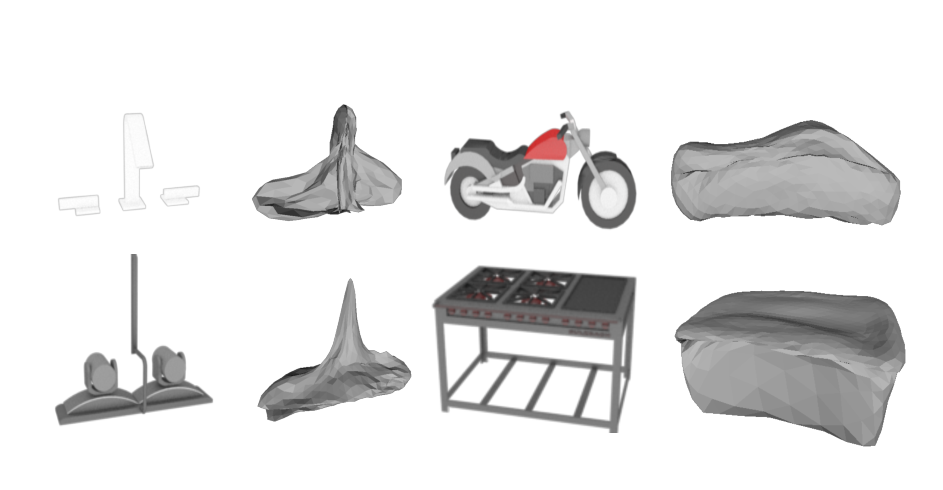
\includegraphics[width=\linewidth]{img/fail/fail1}
	\caption{Failure cases: In some cases, the view angle is adjusted for better exposure of imperfection}
	\label{fig:fail1}
\end{figure*}
\begin{figure}[htbp]
	\centering
	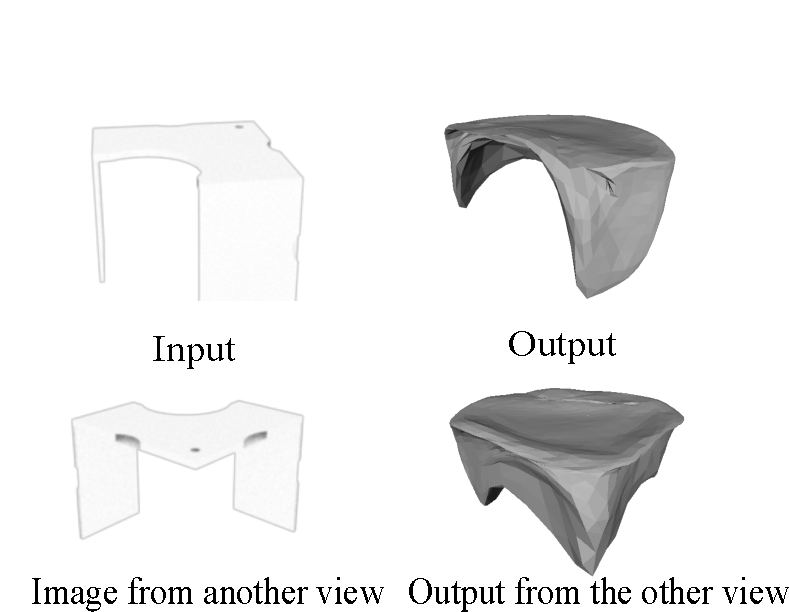
\includegraphics[width=\linewidth]{img/fail/fail2}
	\caption{Failure case: In this case, the network have output an extra leg that doesn't exist for the dresser}
	\label{fig:fail2}
\end{figure}


